\chapter{Implementation}
\label{sec:impl}

This chapter presents the implementation and architecture of stereo vision system presented in this paper.

\section{Architecture Overview}

The stereo vision module in this paper is composed of three main parts: SAD, minimum comparators, and a wrapper, which goes around the previous two that takes in image data and outputs disparity values.

The code for the following sections is located on github under:
\\\path{https://github.com/cccitron/mastersThesis}.

\subsection{Sum of the Absolute Differences Architecture}

Two versions of the SAD algorithm have been implemented in this paper. The first uses a 9x9 window and the other one uses a 7x7 window. Figure~\ref{fig:sadAlg_rtl} shows the top level entity of the SAD implementation used. Both versions have a clocked input (clk\_I) and a one bit data input (data\_I) to notify the algorithm to begin calculating the SAD value. The template\_window\_I and search\_window\_I between the two versions differ in the sense that the number of bytes, 49 or 81, sent to the sadAlgorithm entity are different. The data\_O signal notifies when the calculation is complete and that it is ready for the next set of input. The calculated SAD value is sent out of the entity through sad\_O.

There is a slight variation between the standard SAD algorithm and how it is implemented in this stereo vision system. Instead of subtracting two pixel values and then taking the absolute difference between them, the implementation in this paper finds which corresponding pixel has a greater value and then sends the two pixels to the subtracter based on that. See Appendix~\ref{sec:appdxA} and Appendix~\ref{sec:appdxB} for the code used. The subtracter then takes the greater value and subtracts from it the lesser value and returns the difference, sub. The value sub will always be greater than or equal to zero, which is equal to the absolute difference of the two corresponding pixels. This process was implemented to reduce the complexity by not needing signed values and allowed for the number of bytes used for logic in the algorithm to be reduced since the values no longer need additional bits to account for the signed portion of negative values.

\begin{figure}[h]
	\begin{center}
		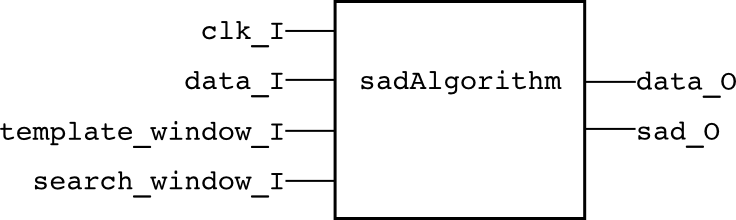
\includegraphics[width=100mm]{figures/sadAlgorithm_rtl.png}
		\captionfonts
		\caption{The top level SAD algorithm implementation.}
		\label{fig:sadAlg_rtl}
	\end{center}
\end{figure}

\subsubsection{State Diagram}

Inside the sadAlgorithm entity from Fig.~\ref{fig:sadAlg_rtl}, the state machine from Figure~\ref{fig:stateMachine} controls the SAD algorithm. The state machine begins at state SO and initializes all the values used in it to 0. It then proceeds to S1 where the state machine remains on standby until data\_I becomes `1'. In S2, the counter starts at 0, the subtraction between corresponding pixel values begins, and on the next clock cycle, the state will be S3. While in S3, the counter is incremented by 1 every clock cycle. S3 is where the SAD algorithm is performed. After the counter is equal to windowSize (7 for the 7x7 and 81 for the 9x9, see Section~\ref{sec:9x9window} and Section~\ref{sec:7x7window} for details) the SAD calculation is complete. The state machine sets data\_O to `1' to notify the SAD wrapper that the calculation is complete and the state moves to S1 and waits for the next set of input.

\begin{figure}[h]
	\begin{center}
		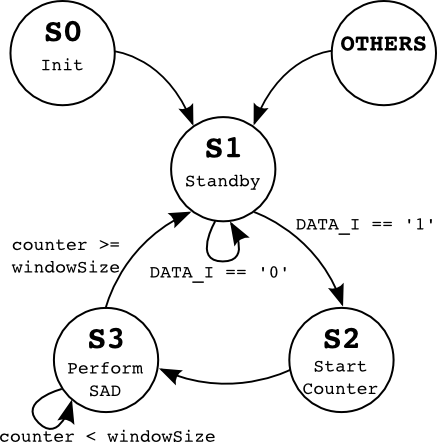
\includegraphics[width=100mm]{figures/stateMachine.png}
		\captionfonts
		\caption{The state machine for implementing the SAD algorithm.}
		\label{fig:stateMachine}
	\end{center}
\end{figure}

\subsubsection{9x9 Window}
\label{sec:9x9window}

The 9x9 window implementation operated with 4 pixels processed in parallel. Every pixel has 16 SAD operations processed in parallel. There are 64 SAD operations total occurring in parallel for the 4 pixels. However, each SAD calculation has a higher degree of serialization than the 7x7 window implementation in order to reduce space to fit on the Atlys board~\cite{atlysBoard}. Figure~\ref{fig:sadAlg9x9} shows a simplified version of this process. Each clock cycle, for 81 cycles, the difference between corresponding pixels is calculated. Beginning one clock cycle after the differences start to be calculated the difference, sub, sum\_out is added to itself and sub. This process also occurs 81 times, one addition each clock cycle. The state machine in Fig.~\ref{fig:stateMachine} stops the calculation for sum\_out after the full SAD value has been summed up.

\begin{figure}[h]
	\begin{center}
		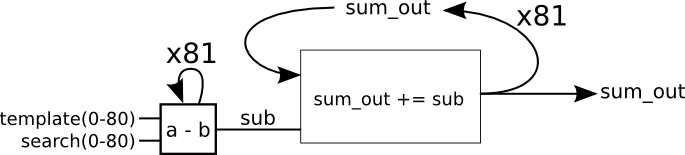
\includegraphics[width=120mm]{figures/sadAlgorithm9x9.png}
		\captionfonts
		\caption{Architecture overview of the SAD algorithm with the 9x9 window implementation.}
		\label{fig:sadAlg9x9}
	\end{center}
\end{figure}

Figure~\ref{fig:sadPipe9x9} illustrates the pipeline used in a SAD calculation in a SAD calculation for the 9x9 window version. It takes 81 clock cycles to take all of the differences between all 81 pairs of pixel values. After the first difference is calculated, the differences can then begin to be summed up. The summing also takes 81 clock cycles and ends one cycle after the last difference is calculated. This results in it taking 82 clock cycles.

\begin{figure}[h]
	\begin{center}
		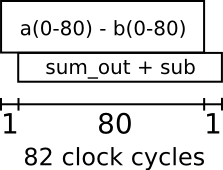
\includegraphics[width=50mm]{figures/sadPipeline9x9.png}
		\captionfonts
		\caption{Pipeline architecture of the SAD algorithm with the 9x9 window implementation.}
		\label{fig:sadPipe9x9}
	\end{center}
\end{figure}

The code for the 9x9 window implementation can be found on github:
\\\path{https://github.com/cccitron/mastersThesis/tree/master/makestuff/libs/libfpgalink-20120621/hdl/fx2/vhdl/sad_simple_reg_9x9}

\subsubsection{7x7 Window}
\label{sec:7x7window}

The 7x7 window implementation operated with 2 pixels processed in parallel. Each pixel has 16 SAD operations processed in parallel. There are only 32 SAD operations occurring in parallel, as opposed to 64 that were performed in parallel in Sec.~\ref{sec:9x9window}. The 7x7 window size has 32 pixels less than the 9x9 version for each window in every SAD calculation. The process was able to utilize a higher degree of parallelization. The increased parallelism takes up more space on the board than the serial version from Sec.~\ref{sec:9x9window}. Figure~\ref{fig:sadAlg7x7} shows a simplified version of this process. Each clock cycle during 7 cycles, the difference, sub, between corresponding pixels is calculated. One clock cycle after the differences begin to be calculated, sum\_out is added to itself and the value sub. This process also occurs 7 times, one set of addition each clock cycle. The state machine in Fig.~\ref{fig:stateMachine} stops the calculation for sum\_out after the full SAD value has been summed up.

The main difference between this implementation and the 9x9 window implementation from Sec.~\ref{sec:9x9window} is that the difference between corresponding pixels is parallelized to calculate 7 absolute differences at once. The dotted box in Fig.~\ref{fig:sadAlg7x7} represents all 7 of the subtraction calculations occurring 7 times in the SAD calculation. Instead of requiring 49 clock cycles to calculate all the differences, it only takes 7 clock cycles. All 7 of the differences that were calculated are added to sum\_out each clock cycle.

\begin{figure}[h]
	\begin{center}
		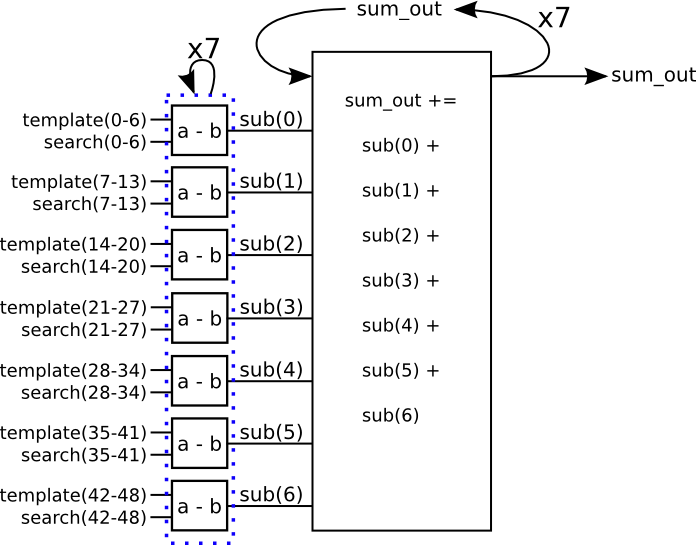
\includegraphics[width=130mm]{figures/sadAlgorithm7x7.png}
		\captionfonts
		\caption{Architecture overview of the SAD algorithm with the 7x7 window implementation.}
		\label{fig:sadAlg7x7}
	\end{center}
\end{figure}

Figure~\ref{fig:sadPipe7x7} shows the pipeline used for the 7x7 window version. It takes 7 clock cycles to take all of the differences between all 49 pairs of pixel values. After the first set of differences is calculated, the differences can begin to be summed up. The summing also takes 7 clock cycles and ends one cycle after the last difference is calculated. This results in a total of 8 clock cycles.

\begin{figure}[h]
	\begin{center}
		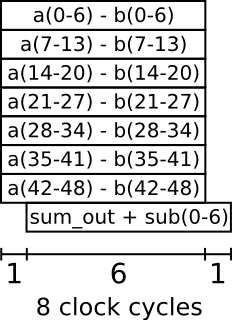
\includegraphics[width=50mm]{figures/sadPipeline7x7.png}
		\captionfonts
		\caption{Pipeline architecture of the SAD algorithm with the 7x7 window implementation.}
		\label{fig:sadPipe7x7}
	\end{center}
\end{figure}

The code for the 7x7 window implementation can be found on github:
\\\path{https://github.com/cccitron/mastersThesis/tree/master/makestuff/libs/libfpgalink-20120621/hdl/fx2/vhdl/sad_parallel_7x7}

\subsection{Minimum Comparator Architecture}

The purpose of the minimum comparator is to find the lowest value of two input values and output the lowest value. The top level implementation of the minimum comparator is shown in Figure~\ref{fig:minComp_rtl}. The process is synchronous, noted by the clock clk\_I. The index, pos0\_I and pos1\_I, of the SAD values sad0\_I and sad1\_I, respectively, ranges from 0 to 15, which gives a disparity range of 16. 

Appendix~\ref{sec:appdxC} shows the code for the minimum comparator. If sad1 is less than sad0, then sad1 and its index, pos1, are returned, otherwise sad0 and pos0 are returned. Using a less than comparison is supposed to take up less hardware than a greater than or equal to comparison~\cite{lessThan}. This is useful because 15 minimum comparators (see Figure~\ref{fig:minComp}) are used for each pixel that is processed in parallel. So 30 minimum comparators are used for the 7x7 window implementation and 60 minimum comparators are used for the 9x9 window implementation. Constructing the minimum comparator in this way accounts for cases where 2 SAD values are equal to each other. The SAD value with the lower index is always assigned to the sad0\_I input and the higher indexed SAD value goes to the sad1\_I input. Therefore, if 2 values are equal, the SAD value with a lower index, and a lower disparity, will be returned. This assumes if two SAD values are equal to each other the value with the index closer to 0 is more likely to be correct.

\begin{figure}[h]
	\begin{center}
		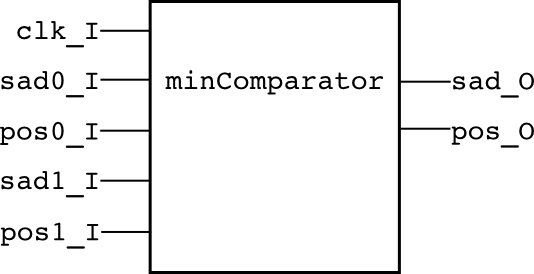
\includegraphics[width=90mm]{figures/minComparator_rtl.png}
		\captionfonts
		\caption{The top level minimum comparator implementation.}
		\label{fig:minComp_rtl}
	\end{center}
\end{figure}

When multiple minimum comparators are put together to create a tree, as shown in Fig.~\ref{fig:minComp}, it is possible to quickly determine which SAD value is the lowest. This process is used to find the index of the lowest SAD value out of the 16 SAD values calculated for each pixel. A normal serial comparison of 16 values would take 15 comparisons, or 15 clock cycles, if one comparison occurred each clock cycle. By having 15 comparators, the number of SAD values needed to be compared can be reduced by half each clock cycle. Using a tree of comparators drops the comparison time from 15 clock cycles to only 4 clock cycles. It is almost a 4 times speed up.

\begin{figure}[h]
	\begin{center}
		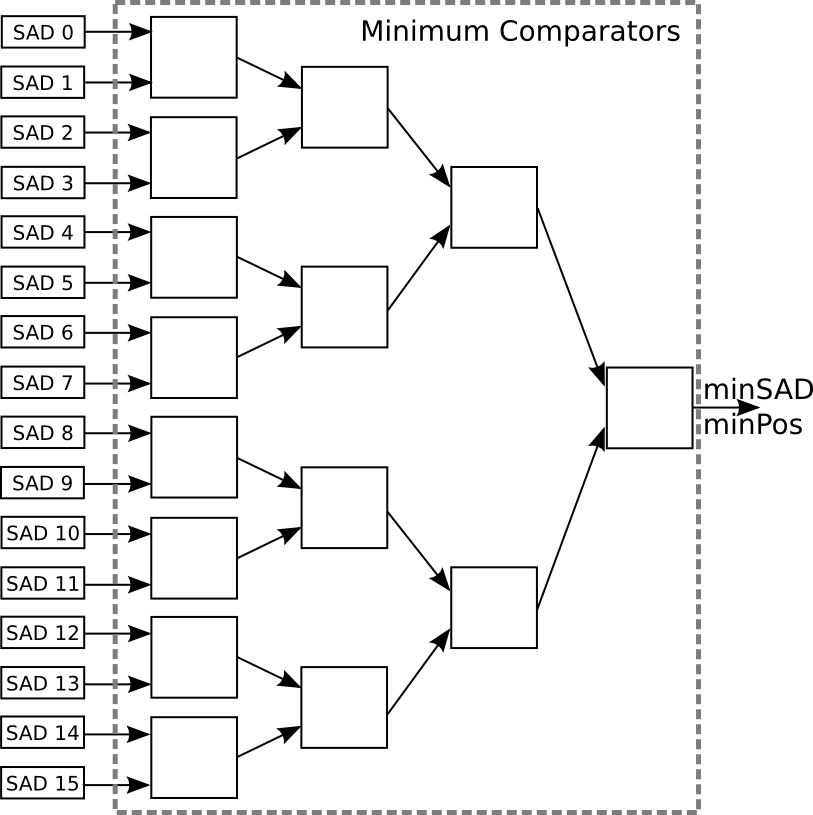
\includegraphics[width=150mm]{figures/minComparator.png}
		\captionfonts
		\caption{The minimum comparator tree designed to quickly find the minimum value and corresponding index out of the 16 SAD values that are calculated for one pixel.}
		\label{fig:minComp}
	\end{center}
\end{figure}

\subsection{SAD Wrapper}

The SAD wrapper is the entity that encompasses the SAD algorithms and minimum comparators. It receives the template image data through templ\_I and receives the search image data through search\_I. The write\_t\_I and write\_s\_I notify the wrapper when new data is actively being sent for the template and search images, respectively. It is designed to allow data from both images to be sent to the wrapper in parallel or serially. The h2fReady\_I and f2hReady\_I are used to communicate when data is being sent to or from the host, the computer, from or to the FPGA. The sw\_I allows the 8 switches on Atlys board to be connected to data that is within the wrapper to be displayed on the 8 LEDs, led\_O. The outputs templ\_O for template image region, search\_O for search image region, sad\_O for the SAD values calculated from the current template and search image regions, and disp\_O that were found from the SAD values are outputted so they can be read, if desired. In the current implementations, templ\_O, search\_O, and sad\_O are used for debugging purposes only while disp\_O is used to create the depth map. See Section~\ref{sec:fpgalink} for how the data is transferred to the computer.

\begin{figure}[h]
	\begin{center}
		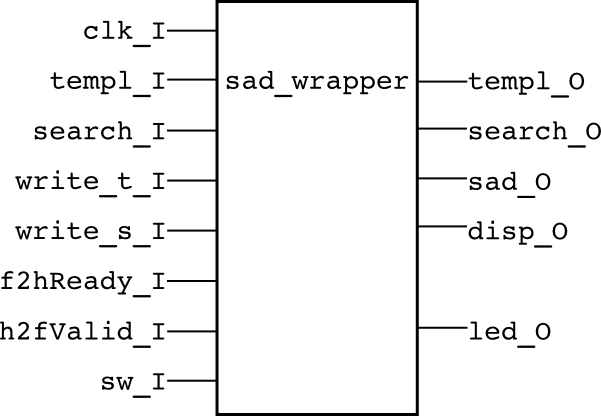
\includegraphics[width=90mm]{figures/sad_wrapper_rtl.png}
		\captionfonts
		\caption{The SAD wrapper that encompasses the SAD algorithm and minimum comparator. It interacts with the top level.}
		\label{fig:sadWrapper_rtl}
	\end{center}
\end{figure}

\subsection{Top Level}

The implementation of the SAD wrapper and its internal entities were designed to be able to work with any FPGA that has enough resources to hold it (see Appendix~\ref{sec:appdxD}). Figure~\ref{fig:topLevel_rtl} shows the SAD wrapper inside a top level entity. The top level gives the SAD wrapper image data and the SAD wrapper gives the top level disparity values. Those values are then transmitted to the computer, see Sec.~\ref{sec:fpgalink} for the communication process. The implementation in Fig.~\ref{fig:topLevel_rtl} represents the 9x9 window implementation. For the 7x7 window implementation, there are only 2 SAD and 2 minimum comparators, as opposed to 4 each.

\begin{figure}[h]
	\begin{center}
		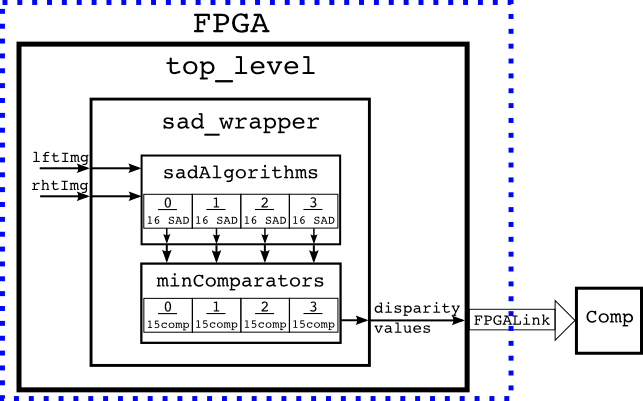
\includegraphics[width=150mm]{figures/top_level_rtl.png}
		\captionfonts
		\caption{The overview of the structure used for implementing the 9x9 window. The 7x7 window has two less SAD and minComp each.}
		\label{fig:topLevel_rtl}
	\end{center}
\end{figure}

\section{FPGALink}
\label{sec:fpgalink}

FPGALink~\cite{fpgalink} was used to facilitate communications between the computer (host) and the FPGA (Atlys board) over USB. An overview of how the FPGALink works between the host and FPGA is shown in Figure~\ref{fig:fpgalink}. The FPGALink has two possible communication modules to choose from, FX2 and EPP. According to~\cite{fpgalink}, FX2 has an observed throughput around 26 MB/s, while EEP has a observed throughput of around 1.26 MB/s. FX2 was used due to its higher throughput.

\begin{figure}[h]
	\begin{center}
		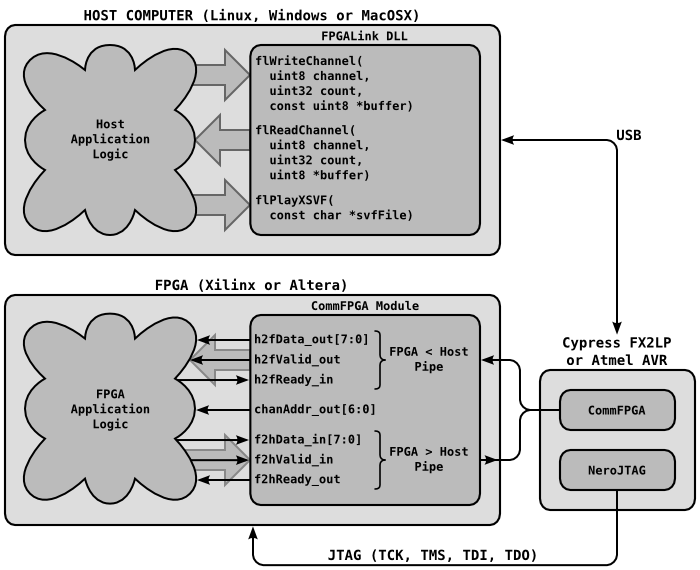
\includegraphics[width=150mm]{figures/fpgalinkOverview.png}
		\captionfonts
		\caption{Overview of FPGALink communications between host computer and FPGA~\cite{fpgalink}.}
		\label{fig:fpgalink}
	\end{center}
\end{figure}
